% Options for packages loaded elsewhere
\PassOptionsToPackage{unicode}{hyperref}
\PassOptionsToPackage{hyphens}{url}
%
\documentclass[
  ignorenonframetext,
]{beamer}
\usepackage{pgfpages}
\setbeamertemplate{caption}[numbered]
\setbeamertemplate{caption label separator}{: }
\setbeamercolor{caption name}{fg=normal text.fg}
\beamertemplatenavigationsymbolsempty
% Prevent slide breaks in the middle of a paragraph
\widowpenalties 1 10000
\raggedbottom
\setbeamertemplate{part page}{
  \centering
  \begin{beamercolorbox}[sep=16pt,center]{part title}
    \usebeamerfont{part title}\insertpart\par
  \end{beamercolorbox}
}
\setbeamertemplate{section page}{
  \centering
  \begin{beamercolorbox}[sep=12pt,center]{part title}
    \usebeamerfont{section title}\insertsection\par
  \end{beamercolorbox}
}
\setbeamertemplate{subsection page}{
  \centering
  \begin{beamercolorbox}[sep=8pt,center]{part title}
    \usebeamerfont{subsection title}\insertsubsection\par
  \end{beamercolorbox}
}
\AtBeginPart{
  \frame{\partpage}
}
\AtBeginSection{
  \ifbibliography
  \else
    \frame{\sectionpage}
  \fi
}
\AtBeginSubsection{
  \frame{\subsectionpage}
}

\usepackage{amsmath,amssymb}
\usepackage{iftex}
\ifPDFTeX
  \usepackage[T1]{fontenc}
  \usepackage[utf8]{inputenc}
  \usepackage{textcomp} % provide euro and other symbols
\else % if luatex or xetex
  \usepackage{unicode-math}
  \defaultfontfeatures{Scale=MatchLowercase}
  \defaultfontfeatures[\rmfamily]{Ligatures=TeX,Scale=1}
\fi
\usepackage{lmodern}
\ifPDFTeX\else  
    % xetex/luatex font selection
\fi
% Use upquote if available, for straight quotes in verbatim environments
\IfFileExists{upquote.sty}{\usepackage{upquote}}{}
\IfFileExists{microtype.sty}{% use microtype if available
  \usepackage[]{microtype}
  \UseMicrotypeSet[protrusion]{basicmath} % disable protrusion for tt fonts
}{}
\makeatletter
\@ifundefined{KOMAClassName}{% if non-KOMA class
  \IfFileExists{parskip.sty}{%
    \usepackage{parskip}
  }{% else
    \setlength{\parindent}{0pt}
    \setlength{\parskip}{6pt plus 2pt minus 1pt}}
}{% if KOMA class
  \KOMAoptions{parskip=half}}
\makeatother
\usepackage{xcolor}
\newif\ifbibliography
\setlength{\emergencystretch}{3em} % prevent overfull lines
\setcounter{secnumdepth}{-\maxdimen} % remove section numbering


\providecommand{\tightlist}{%
  \setlength{\itemsep}{0pt}\setlength{\parskip}{0pt}}\usepackage{longtable,booktabs,array}
\usepackage{calc} % for calculating minipage widths
\usepackage{caption}
% Make caption package work with longtable
\makeatletter
\def\fnum@table{\tablename~\thetable}
\makeatother
\usepackage{graphicx}
\makeatletter
\def\maxwidth{\ifdim\Gin@nat@width>\linewidth\linewidth\else\Gin@nat@width\fi}
\def\maxheight{\ifdim\Gin@nat@height>\textheight\textheight\else\Gin@nat@height\fi}
\makeatother
% Scale images if necessary, so that they will not overflow the page
% margins by default, and it is still possible to overwrite the defaults
% using explicit options in \includegraphics[width, height, ...]{}
\setkeys{Gin}{width=\maxwidth,height=\maxheight,keepaspectratio}
% Set default figure placement to htbp
\makeatletter
\def\fps@figure{htbp}
\makeatother

\makeatletter
\@ifpackageloaded{caption}{}{\usepackage{caption}}
\AtBeginDocument{%
\ifdefined\contentsname
  \renewcommand*\contentsname{Table of contents}
\else
  \newcommand\contentsname{Table of contents}
\fi
\ifdefined\listfigurename
  \renewcommand*\listfigurename{List of Figures}
\else
  \newcommand\listfigurename{List of Figures}
\fi
\ifdefined\listtablename
  \renewcommand*\listtablename{List of Tables}
\else
  \newcommand\listtablename{List of Tables}
\fi
\ifdefined\figurename
  \renewcommand*\figurename{Figure}
\else
  \newcommand\figurename{Figure}
\fi
\ifdefined\tablename
  \renewcommand*\tablename{Table}
\else
  \newcommand\tablename{Table}
\fi
}
\@ifpackageloaded{float}{}{\usepackage{float}}
\floatstyle{ruled}
\@ifundefined{c@chapter}{\newfloat{codelisting}{h}{lop}}{\newfloat{codelisting}{h}{lop}[chapter]}
\floatname{codelisting}{Listing}
\newcommand*\listoflistings{\listof{codelisting}{List of Listings}}
\makeatother
\makeatletter
\makeatother
\makeatletter
\@ifpackageloaded{caption}{}{\usepackage{caption}}
\@ifpackageloaded{subcaption}{}{\usepackage{subcaption}}
\makeatother
\ifLuaTeX
  \usepackage{selnolig}  % disable illegal ligatures
\fi
\usepackage{bookmark}

\IfFileExists{xurl.sty}{\usepackage{xurl}}{} % add URL line breaks if available
\urlstyle{same} % disable monospaced font for URLs
\hypersetup{
  pdftitle={PointedSDMs Workshop},
  pdfauthor={Philip Mostert, Ron Tugonov, Kwaku Adjei, Bob O'Hara},
  hidelinks,
  pdfcreator={LaTeX via pandoc}}

\title{PointedSDMs Workshop}
\author{Philip Mostert, Ron Tugonov, Kwaku Adjei, Bob O'Hara}
\date{2024-07-13}
\institute{ISEC 2024, Swansea, Wales}

\begin{document}
\frame{\titlepage}

\begin{frame}
\begin{block}{Who We Are}
\phantomsection\label{who-we-are}
\begin{columns}[T]
\begin{column}{0.25\textwidth}
\begin{figure}[H]

{\centering 
\includegraphics{Images/BobOH.jpg}

}

\caption{Bob O'Hara}

\end{figure}%
\end{column}

\begin{column}{0.25\textwidth}
\begin{figure}[H]

{\centering 
\includegraphics{Images/Philip.jpg}

}

\caption{Philip Mostert}

\end{figure}%
\end{column}

\begin{column}{0.25\textwidth}
\begin{figure}[H]

{\centering 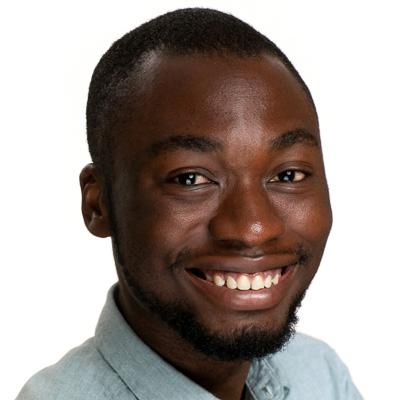
\includegraphics{Images/Kwaku.jpg}

}

\caption{Kwaku Adjei}

\end{figure}%
\end{column}

\begin{column}{0.25\textwidth}
\begin{figure}[H]

{\centering 
\includegraphics{Images/RonT.jpg}

}

\caption{Ron Togonov}

\end{figure}%
\end{column}

\begin{frame}{Presentation 1: What are ISDMs?}
\phantomsection\label{presentation-1-what-are-isdms}
\end{frame}
\end{columns}

::::
\end{block}
\end{frame}

\begin{frame}{Why Integrate Data?}
\phantomsection\label{why-integrate-data}
\begin{block}{Data are messy}
\phantomsection\label{data-are-messy}
\includegraphics{Images/LepsNA.gif}
\end{block}

\begin{block}{Data are messy}
\phantomsection\label{data-are-messy-1}
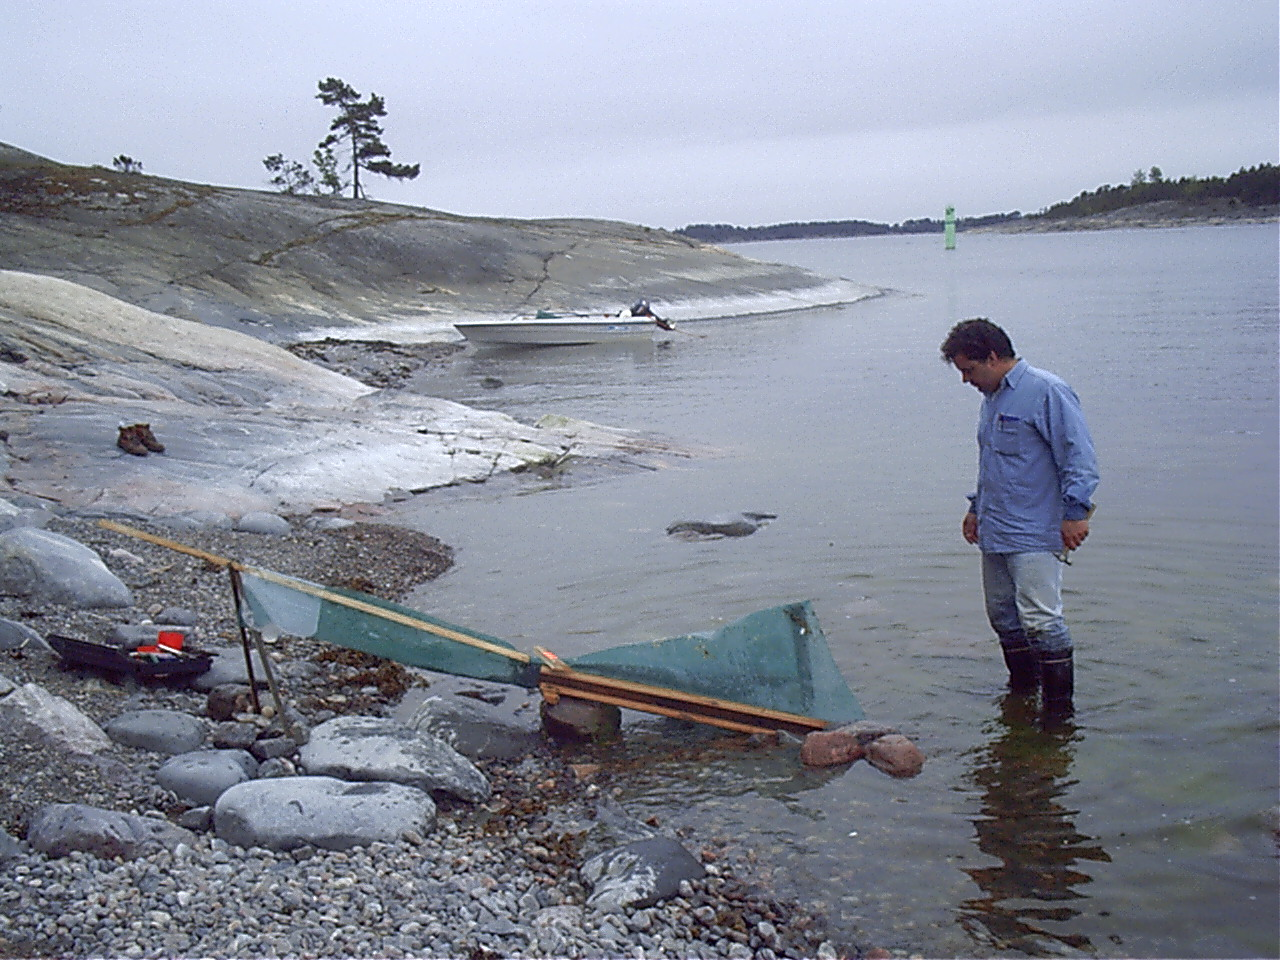
\includegraphics{Images/JohanTrap.JPG}
\end{block}

\begin{block}{Merge data}
\phantomsection\label{merge-data}
\begin{figure}[H]

{\centering 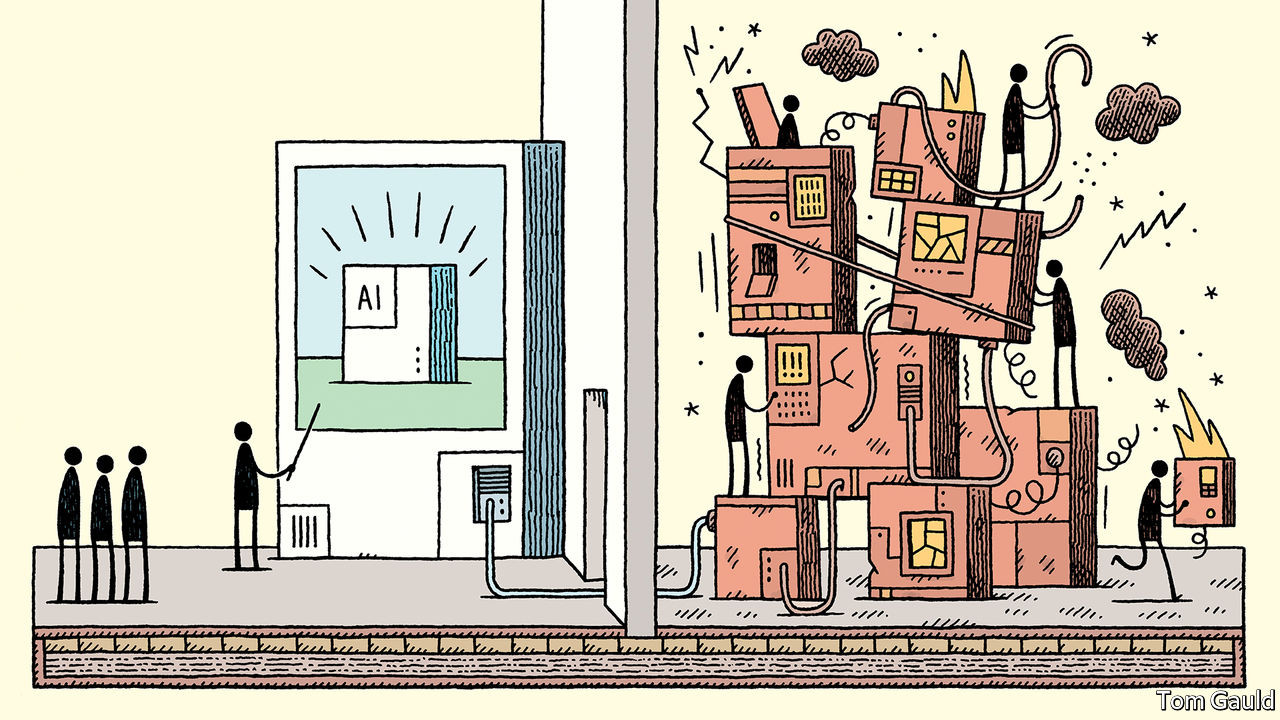
\includegraphics{Images/TomGaiuuldAI.jpg}

}

\caption{Cartoon by Tom Gauld: https://www.tomgauld.com/}

\end{figure}%
\end{block}
\end{frame}

\begin{frame}{The Model Framework}
\phantomsection\label{the-model-framework}
\begin{block}{The Pieces}
\phantomsection\label{the-pieces}
\begin{itemize}
\tightlist
\item
  \(P(Y_d | \lambda(\mathbf{s}), \theta_d)\): One observation model per
  data set
\item
  \(P(\lambda(\mathbf{s}))\) One process model
\end{itemize}

Full likelihood

\[
L(Y | \theta_d) = P(\lambda(\mathbf{s})) \prod_{d=1}^{M}P(Y_d | \lambda(\mathbf{s}), \theta_d)
\]
\end{block}

\begin{block}{Point Processes}
\phantomsection\label{point-processes}
Point processes are defined on a continuous space

\begin{itemize}
\tightlist
\item
  intensity \(\lambda({\bf s})\)
\end{itemize}

For an area \(A\), mean number of points in area is

\[
\mu_A = \int_A \lambda({\bf s}) d{\bf s}
\]

Actual number follows a Poisson distribution with mean \(\mu_A\)
\end{block}

\begin{block}{Observation processes}
\phantomsection\label{observation-processes}
\begin{itemize}
\tightlist
\item
  Counts: \(N_A \sim Poisson(p \mu_A)\)
\item
  Presence/Absence: \((N_A >0) \sim Bern( 1-e^{-p \mu_A})\) (=cloglog)
\item
  Points: Thinned point process
\end{itemize}
\end{block}
\end{frame}

\begin{frame}{Why have a package?}
\phantomsection\label{why-have-a-package}
\begin{itemize}
\tightlist
\item
  not easy to code from scratch
\item
  lots of pieces that are the same between models
\item
  models are modular, so a package can help piece them together
\end{itemize}
\end{frame}

\begin{frame}[fragile]{What we will do today}
\phantomsection\label{what-we-will-do-today}
\begin{itemize}
\tightlist
\item
  Exercise 1: your first model with \texttt{PointedSDMs}
\item
  Presentation 2: What you just did (and why)
\item
  Exercise 2: A bit more modelling: how to change the model
\item
  Presentation 3: Multi-species models
\item
  Exercise 3: Multi-species models
\item
  Discussion and wrapping up
\end{itemize}
\end{frame}

\begin{frame}{Exercise 1: Your first (and second?) model}
\phantomsection\label{exercise-1-your-first-and-second-model}
First: pull from the \emph{Github} repository:
\emph{https://github.com/PhilipMostert/PointedSDMs}

devtools::install\_github(`PhilipMostert/PointedSDMs@main')

(this is more recent than CRAN)

Then pull the workshop: \emph{PhilipMostert/PointedSDMs\_Workshop.}

The first exercise is here:

\emph{https://github.com/PhilipMostert/PointedSDMs\_Workshop/blob/main/Exercises/SetophagaExercise1.html}
\end{frame}



\end{document}
